%input macros (i.e. write your own macros file called MacroFile1.tex)
%\newcommand{\PdfPsText}[2]{
  \ifpdf
     #1
  \else
     #2
  \fi
}

\newcommand{\IncludeGraphicsH}[3]{
  \PdfPsText{\includegraphics[height=#2]{#1}}{\includegraphics[bb = #3, height=#2]{#1}}
}

\newcommand{\IncludeGraphicsW}[3]{
  \PdfPsText{\includegraphics[width=#2]{#1}}{\includegraphics[bb = #3, width=#2]{#1}}
}

\newcommand{\InsertFig}[3]{
  \begin{figure}[!htbp]
    \begin{center}
      \leavevmode
      #1
      \caption{#2}
      \label{#3}
    \end{center}
  \end{figure}
}


%%% Local Variables: 
%%% mode: latex
%%% TeX-master: "~/Documents/LaTeX/CUEDThesisPSnPDF/thesis"
%%% End: 


 \documentclass[oneside,12pt]{Classes/CUEDthesisPSnPDF}


\ifpdf
    \pdfinfo { /Title  (CUED PhD and MPhil Thesis Classes)
               /Creator (TeX)
               /Producer (pdfTeX)
               /Author (Fangde Liu)
               /CreationDate (D:20030101000000)  %format D:YYYYMMDDhhmmss
               /ModDate (D:20030815213532)
               /Subject (Adaptive Motion Synthesis)
               /Keywords (PhD, Thesis)}
    \pdfcatalog { /PageMode (/UseOutlines)
                  /OpenAction (fitbh)  }
\fi

\title{Adaptive Motion Synthesis}

\ifpdf
  \author{\href{mailto:fliu@bmth.ac.uk}{Fangde Liu}}
  \collegeordept{\href{http://www.eng.cam.ac.uk}{Department of Engineering}}
  \university{\href{http://www.cam.ac.uk}{University of Cambridge}}
% insert below the file name that contains the crest in-place of 'UnivShield'
  \crest{
\includegraphics[width=30mm]{UnivShield}}
\else
  \author{Fangde Liu}
  \collegeordept{National Center For Computer Animation, Media School}
  \university{Bournemouth University}
% insert below the file name that contains the crest in-place of 'UnivShield'
  \crest{
\includegraphics[bb = 0 0 292 336, width=30mm]{UnivShield}}
\fi
%
% insert below the file name that contains the crest in-place of 'UnivShield'
% \crest{\IncludeGraphicsW{UnivShield}{40mm}{14 14 73 81}}
%
%\renewcommand{\submittedtext}{change the default text here if needed}
\degree{Doctor of Philosophy}
\degreedate{Yet to be decided}

% turn of those nasty overfull and underfull hboxes
\hbadness=10000
\hfuzz=50pt

% Put all the style files you want in the directory StyleFiles and usepackage like this:
\usepackage{StyleFiles/watermark}

% Comment out the next line to get single spacing
\onehalfspacing

\begin{document}

%\language{english}

% A page with the abstract on including title and author etc may be
% required to be handed in separately. If this is not so, then comment
% the below 3 lines (between '\begin{abstractseparte}' and 
% 'end{abstractseparate}'), normally like a declaration ... needs some more
% work, mind as environment abstracts creates a new page!
% \begin{abstractseparate}
%   
% Thesis Abstract -----------------------------------------------------


%\begin{abstractslong}    %uncommenting this line, gives a different abstract heading
\begin{abstracts}        %this creates the heading for the abstract page

Generating natural-looking motions for virtual characters is a challenging research topic.
It becomes even harder when generating adaptive motions interacting with the environment. 
Current methods are tedious, cost long computational time and fail to capture natural looking features.

This report proposes an efficient method of generating natural-looking motion based upon a new motor control theory.
The principal idea is motor repertoire is made up of a limited number of elements. Motor control basically connect the basic motion primitives together just like connecting alphabets into sentences.

we propose principle of motor control is not feedback based, they should by model as topology conjugacy.
During motion adaptation, neural system tweaks the basic mechanical system to form an analogous dynamic system that meets constraints and purpose.

When animals adapt their motion, some properties are maintained, which are called motor invariant.
Motion Primitives are identified by the qualitative properties, for which we use the mathematical tools of differential topology.
Tweaking of the motion primitives is model as Symmetry Preserved Transformation, for which we use lie group theory.



Following our idea, we generate adaptive natural looking motion with very little computational costs.
\end{abstracts}
%\end{abstractlongs}


% ----------------------------------------------------------------------


%%% Local Variables: 
%%% mode: latex
%%% TeX-master: "../thesis"
%%% End: 


% \end{abstractseparate}




% Using the watermark package which is in StyleFiles/
% and to remove DRAFT COPY ONLY appearing on the top of all pages comment out below line
%\watermark{DRAFT COPY ONLY}


\maketitle

%set the number of sectioning levels that get number and appear in the contents
\setcounter{secnumdepth}{3}
\setcounter{tocdepth}{3}

\frontmatter % book mode only
\pagenumbering{roman}
% Thesis Dedictation ---------------------------------------------------

\begin{dedication} %this creates the heading for the dedication page

This work is dedicated to my loving parents, who are always ready to sacrifice everything for me.


\end{dedication}

% ----------------------------------------------------------------------

%%% Local Variables: 
%%% mode: latex
%%% TeX-master: "../thesis"
%%% End: 

% Thesis Acknowledgements ------------------------------------------------


%\begin{acknowledgementslong} %uncommenting this line, gives a different acknowledgements heading
\begin{acknowledgements}      %this creates the heading for the acknowlegments


And I would like to acknowledge ...


\end{acknowledgements}
%\end{acknowledgmentslong}

% ------------------------------------------------------------------------

%%% Local Variables: 
%%% mode: latex
%%% TeX-master: "../thesis"
%%% End: 


% Thesis Abstract -----------------------------------------------------


%\begin{abstractslong}    %uncommenting this line, gives a different abstract heading
\begin{abstracts}        %this creates the heading for the abstract page

Generating natural-looking motions for virtual characters is a challenging research topic.
It becomes even harder when generating adaptive motions interacting with the environment. 
Current methods are tedious, cost long computational time and fail to capture natural looking features.

This report proposes an efficient method of generating natural-looking motion based upon a new motor control theory.
The principal idea is motor repertoire is made up of a limited number of elements. Motor control basically connect the basic motion primitives together just like connecting alphabets into sentences.

we propose principle of motor control is not feedback based, they should by model as topology conjugacy.
During motion adaptation, neural system tweaks the basic mechanical system to form an analogous dynamic system that meets constraints and purpose.

When animals adapt their motion, some properties are maintained, which are called motor invariant.
Motion Primitives are identified by the qualitative properties, for which we use the mathematical tools of differential topology.
Tweaking of the motion primitives is model as Symmetry Preserved Transformation, for which we use lie group theory.



Following our idea, we generate adaptive natural looking motion with very little computational costs.
\end{abstracts}
%\end{abstractlongs}


% ----------------------------------------------------------------------


%%% Local Variables: 
%%% mode: latex
%%% TeX-master: "../thesis"
%%% End: 



\tableofcontents
\listoffigures
\printnomenclature  %% Print the nomenclature
\addcontentsline{toc}{chapter}{Nomenclature}

\mainmatter % book mode only
%%% Thesis Introduction --------------------------------------------------
\chapter{INTRODUCTION}
\label{chap:intro}

\graphicspath{{Introduction/IntroductionFigs/EPS/}{Introduction/IntroductionFigs/}}
\nomenclature[z1]{\cms}{Character Motion Synthesis}
\nomenclature[z2]{\cpg}{Central Pattern Generator}
\nomenclature[z3]{\dof}{Degree of Freedom}
\nomenclature[z2]{\moit}{Motor Invariant Theory}

\section{The Challenge}
Character Motion Synthesis (\cms) research aims at generating motion for virtual characters.
It is a topic of significant value in terms of theory and application. 
Besides major applications in the media industry, where both computer games and animation films depend heavily upon character motion for storytelling, 
current research also has applications in user interface design, psychology, sports and medicine.

The challenge of \cms  is not to make characters move, but  to make them lifelike. 
Underlying this challenge is the marvellous human ability of motion perception. 
In real life,people's motion is very similar, yet individuals vary considerably.
From the varieties in motion details, humans can infer mental states, health conditions or the surrounding environment.
%\note{uncanny valley}
Human motion perception has some very peculiar properties.
When wathing a film with computer generated characters, some awkward artefacts are spotted instantly even though they are physically feasible, while many physically impossible motions are accepted as realistic and entertaining. 

%nautral looking

Nowadays in industry, high quality motions are mainly generated manully. 
Very often, characters are complex and contain a large number of joints, making animation tedious work.
To make it worse, reusing motion animation is also difficult and prone to artefacts.
Therefore high level animation tools are badly needed. 

%\note{Do An introduction for physicall based animaiton?}


Real life motions interact extensively with the environment.
Currently, the most important research endeavour is the physics based approach.
Besides  the addition of the dynamic interactive responses, it is  expected that the elimination of  artefacts that violates physics  will make motions more natural looking.
However, this paradigm faces many difficulties:
dynamics of biological systems are much more complex than artificial systems,  attempts to dynamically simulate biological system face prohibitive  computational costs and modelling difficulties.
In fact, such problems have already been identified by biological researchers.







Motor Control and Motion Perception are close related.
Difficulties in \cms reflect the inferiority of artificial control method.
The peculiarity of motion perception and control suggests  biological systems may adopt a different principle.
To generate natural looking motion, it is worthwhile to synthesize motion following the biological motor control principle. 
This thesis is founded on new ideas from biological research.

 

\section{Agile Animals}
%\note{Underlying these problems} is our misunderstanding of animal motions.
Although animals have fascinated us for thousands of years, we still do not fully understand how they move.
Animals are very different from artificial machines and such comparisons may reflect the  biological motor control principle.
%some basic questions of motor control and motion perception remain open. 
%And answers to such questions become even more valuable nowadays. 
%Advance in this topic will greatly influence the biology, robotic engineering even intelligent research.
%\note{The difference between biological motor system}

%The paradoxes is even human are good at motor control and motion perception; human still don’t have an idea of how we move and how we perceive motion.
%Before going into details into the research ideas, we first review some puzzles troubles the foundation of CMS. 
\begin{itemize}
\HiItem {Degrees of freedom ({\dof}s)}.
From a mechanical perspective, animals have many more {\dof}s than their artificial counterparts.
An artificial ship can be approximated by a simple rigid body; whereas the flexible vertebrae of a finsih is made up of tens of {\dof}s.


In principle, the extra {\dof}s allows for more variations in adapting the environment. 
However, for the control system, too many extra {\dof}s are a disaster because of the computational burden. 
For a human to take one step,  the neural system controls more than $600$ muscles.
Even with nowadays computer, solving the dynamics directly would spend thousands of hours.

 
\HiItem {Versatility}
Most artificial machines are designed with a single purpose,while animals are capable  of unlimited tasks.
Many biological functions which are often neglected by \cms research, such as feeding, breeding, language and vision, depend on motor control. 
Besides walking, swimming and many other styles of locomotion, we utilize many tools, such as cars, skates, bicycles and tennis rackets.

Following traditional control methods, it seems that unlimited resources need to be  allocated for motor control, while biological research shows motor control requires very few mental resources.

\HiItem{Performance}
Although the problem of biological motor control is more complex, the resulting performance surpasses artificial machines in many aspects.
Natural motions are more
\begin{enumerate} 

\HiItem{Robust:}
A human can maintain walking stability on rough terrains which would be inaccessible for vehicles.

\HiItem{Manoeuvrability and speed:}
Typical modern aeroplanes  travel at a maximum of $32\: body\: length/sec$ and yaw at $720\: deg/sec$.
While pigeons may travel at $75 \:body\: length / sec$, yaw at about  $5000 \: deg/sec$.

\HiItem{Energy Efficiency:}
The energy consumed by a human walking is only $5\%$ of that for the world famous humanoid ASIMO.
\end{enumerate}

\end{itemize}



%For computer animation research, the key principle is we should know the things we animate.
%Natural motion system has many valuable properties which are not captured by current motion synthesis methods.
%\begin{itemize} 
% \HiItem{robust}
%Natural motions are adaptive to the changes in the environment or body conditions. 
%A common example is human locomotion. 
%Walking on different terrains will exhibit different gait while the balance is maintained. 
%
%\HiItem{speedy}
%Some motions of animals are very fast, honey birds may vibrate their wings in kHz.
%The astonishment is to the speed of motion, more puzzling is that the neural system can solve the complex motion control problem in such a short time. 
%When an animal avoids obstacles at very high running speed, 
%it must continue its running, make a turning and keep balance at the same time. 
%It seems easy for the neural system to plan complicate motions.
%\HiItem{Energy Efficient}
%Natural Motions are energy efficient.
%In theory, this idea is supported by Darwin's Theory of Evolution.
%But animals spent far less energy than our expectation.
%An example is that the energy consumed by human walking is only 5\% of that for a robot of the same scale.
%\end{itemize}

\section{Motor Invariant Theory}
\subsection{Utilizing Natural Dynamics}
Biological Motor Control has achieved a delicate balance of robustness, controllability and energy efficiency.
The real-time performance may further suggest that the biological method  is simple and requires little computational load.
These are the dreaming properties for \cms research and  the explanation that how biological system achieve this  forms the genesis of this thesis.



Interactions between the body and environment pose  complex dynamic problems for motor control.
In most \cms research studies, such natural dynamics are treated as noises or perturbations to motion planning, and the  effects  of natural dynamics are cancelled by control effort.
However from an evolutionary perspective, the mechanical structures are a product of natural selection which has evolved alongside with the environment for millions of years. 
These structures are an advantages rather than a handicap. 
Without the need to consider stability, energy efficiency and real-time constraints, motor control can be easily achieved if the motion is totally governed by natural dynamics and requires no control effort.
A new idea is that motor control is based on natural dynamics.
The neural system plays a minor role in planning; it simply utilizes natural dynamic properties.

Motor Invariant Theory (\moit)  proposes  how to utilize the natural dynamics in a systematic manner.








\subsection{Motor Invariant Theory}
%In this thesis, we propose different idea towards motor control and motion synthesis.
%In this research, we propose a different motion synthesis method based on a different motor control theory.
%
%An insightful discovery is that motor control can be “easy”.
%For some situation, some tasks mainly explore the properties of the body and environment and can be achieved with little control effort.
%In nature, we don’t finish difficult motion tasks, we select many easy motion tasks that we are good at, connect or modify them for our special purpose.
%
%The “easy” tasks are called motion primitives; they are the basic elements of our motor ability. 
%When we modify the motion primitives, some valuable properties of motion primitives are kept unchanged, and the maintained properties are called motor invariants.
%
%The inspiration of our idea comes from related biological research, which covers biomechanics and neural science.





This thesis proposes a new idea for the underlying reason for superiority of biological motor control.
The insight is that in the process of motion adaption, some valuable properties of natural dynamics are kept invariant.
The conjecture is that:  instead of detecting and cancelation all kinds of perturbations, biological motor control relies on the invariance of natural dynamic properties for motion success.
This is \emph{Motor Invariant Theory(\moit)}.


\moit incorporates the motion primitive conjecture.
In dynamics, invariant properties are stable properties. 
From a dynamic perspective, not all the motions generated by natural dynamics are stable, only the stable ones are utilized and treated as the templates.
In dynamics, invariant properties are stable properties.
From a dynamic perspective, not all the motions generated by natural dynamics are stable, only a few are stable, which can be utilized motion templates and become motion primitives.
The remaining question is how the motor control system utilizes the templates to synthesize motion.

The \moit propose that when facing a new situation, human don't solve motor control from ground up,
motor control system utilizes successful experience in similar situations.
In dynamics, adapted motions are qualitative the same with the motion primitives or templates.
In dynamics, adapted motions are qualitative the same with the motion primitives or templates, and there is a one-one mapping relationship between the adapted motion and the motion primitive.
This similarity in dynamics is topological conjugacy. 

In dynamic \cms research, a motion is represented by  a curve  $x(t)$ parameterized by $t$.
$x(t)$ is the solution to the equation (Equation ~\ref{eq:BodyEnvDym}) that describes the body and environment dynamics.
\begin{equation}
\dot{x}=F(x)
\label{eq:BodyEnvDym}
\end{equation}


To illustrate adaptation, we define a transformation $T$ that acts on the space of $x$.
\[
\tilde{x}=T(x)
\]

In this way, each equation can be described in two coordinate systems: one by $x$ and one by $\tilde{x}$.
As an example, Equation ~\ref{eq:EQtransform} is describes the same dynamics as  Equation ~\ref{eq:tranformedEQ} in a different coordinate system.
then we can obtain two equations in  the transformed state $\tilde{x}$ ( )and original state $x$(Equation ~\ref{eq:EQtransform}).

\begin{equation}
\dot{\tilde{x}}=F(\tilde{x})
\label{eq:tranformedEQ}
\end{equation}

\begin{equation}
\dot{x}=\tilde{F}(x)
\label{eq:EQtransform}
\end{equation}

Since such two equations describe the same motion in different coordinate systems, the solution to one equation can be achieved by transforming the solution to the other equation.
Supposing $x'(t)$ is the solution to Equation~\ref{eq:EQtransform} and $\tilde{x}(t)$ is the solution to the Equation~\ref{eq:tranformedEQ}, then we have
\[
x'(t)=T^{-1}(\tilde{x}(t))
\]
Equation~\ref{eq:tranformedEQ} and Equation~\ref{eq:BodyEnvDym} are the same, thus: 
\[
\tilde{x}(t)=x(t)
\]
Then we have
\[
x'(t)=T^{-1}(x(t))
\]

By transformation, we obtained a new motion $x'(t)$ from $x(t)$.





%if we substitue x=f(x,t) into (1).
%we can express equation (2) interm of (x,t,x)
%\dot(x)=F'(x).
%then the solution of the equation becomes 
%x2(t)=(x)t=f-1(xt)
%
%
The  transformation method has many advantages: it is much less computational expensive and keeps many important properties untouched.
For example, if the original dynamics is stable, then the transformed dynamics is also stable. 
%
If there exists continuous one-one mapping between the two dynamic equations, then the two are \emph{topological conjugate}.
This relationship is presented by $F \simeq \tilde{F}$.
$F$ and $\tilde{F}$ are called \emph{analogous systems},, which share the same topology structure.
The existence of one-one mapping is the necessary and sufficient condition for topological conjugate, thus there are two basic approaches for motion adaption.
Transformation can be specified explicitly or implicitly by maintaining the topology.



If the perturbation does not violate the topology, the corresponding one-one mapping will modify the motion without changing it qualitatively.
In dynamics,the topology preserving ability is an intrinsic property of many dynamic systems:
\emph{structural stability}.
One strategy of motor control is to enhance the structural stability. 
With this approach, the qualitative property is preserved and there exists a one-one mapping relationship, but finding out details of motion will be difficult or computational expensive.
Therefore this approach is qualitative.

In \moit,this approach models the involuntary motion adaptation which is low level function of neural control system.
The topological structure is one important property should be kept invariant, thus become a motor invariant in \moit: the \emph{Global Motor Invariant}.






Also if the transformation is known, then the two systems must be topological equivalent.
This method  modifies motion with precision and \moit applies this idea for high level voluntary motor control.
In many situations, to achieve desired transform $T$, control effort needs to be applied.
For this method, choosing a proper transformation $T$ is the most challenging  question.

In \moit, selection of $T$ is based on two principles.
\begin{itemize}
\item
Parameters of transformation $T$ should be easy to detect and formulated, which meets the biological sensing and computational constraints. 

\item 
The transformation $T$ should be energy efficient.
For differential dynamic system, some transformation explores the natural dynamics and requires little or no energy input.
\end{itemize}
Some quantitative properties will be unchanged during transformation, which are called \emph{Local Motor Invariant}






%the stability of the orignal system is known.
%if possible, we always try to tranform the stable motion.
%To this end motor control are applied to execute the transformation
%
%
%
%these two ideas have pros and cons.
%The first method maintail the qualitative properties, but details of motion can not be controlled precisely.
%if the second method is applied, given the transformation, the resulting motion can be know, while but to carried out such transformation, controll effort may needed.
%
%




Although new mathematical language seems obscure at first glimpse, the properties that the mathematical language describes are universal in physical world, with or without life.
The underlying idea is intuitive and can be explained well through commonly observed phenomena.



\subsection{The Floating Ship: An example of Stability}
The floating ship  example shows the idea of structural stability and topological conjugacy.
In real life, ships floating on the wave are typically taller than they are wide,as shown in Figure~\ref{fig:ShipFloating}.
An interesting  question is how the ship maintains its posture.

Through analysing the topology and structural stability, we see that it is trivial to maintain posture.
This conclusion applies to different ships since their dynamics are qualitative the same, or topological conjugate.


\subsubsection*{Dynamics}

\begin{figure}[!htbp]
  \begin{center}
    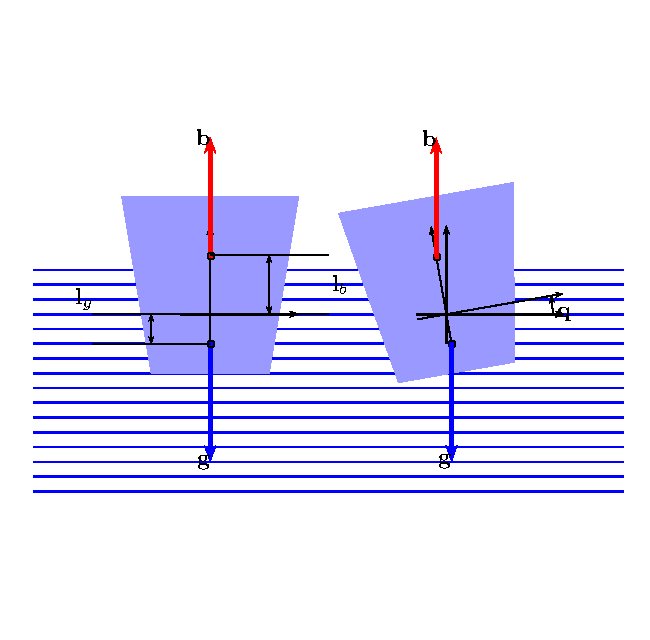
\includegraphics{ShipExample}
    \caption{The Floating Ship Example}
    \label{fig:ShipFloating}
  \end{center}
\end{figure}

The sway motion of the ship shown in Figure ~\ref{fig:ShipFloating} can be described by Equation~\ref{eq:shipflow}
\begin{equation}
\label{eq:shipflow}
J\ddot{q}+d\dot{q}=\tau(q)_{g}+\tau(q)_{b}+\tau_{u}
\end{equation}


where $q$ is the swaying angle.
$J$ is the inertia,  
$d$ is the damping coefficient,
and $\tau_{g}$,$\tau_{b}$,$\tau_{u}$ are the corresponding the torques of gravity, buoyancy and external control.

When a ship is on the sea, the motion is governed by the two forces, the buoyancy $b$ and gravity $g$.
When $\tau_{u}=0$,  the dynamics is becomes governed by its natural property.
Such a system is \emph{autonomous}.

To make it consistent with discussions in following chapters, Equation~\ref{eq:shipflow} is reformulated.
Defining the \emph{state} variable $\state=[q,\qd]$, then Equation~\ref{eq:shipflow} becomes
\[
\dot{\state}=F_{J,d}(\state)+Du
\]

where 
$F$ is a function of $\state$, the subscripts~$J$ and~$d$ are \emph{system parameters},
$D$ is a matrix, which describes how the control effort is applied,
and $u$ is \emph{control input}, for this example $u$ is $\tau_{u}$



\subsubsection*{Equilibrium Postures}
A ship will only rest when $\tau_{g}+\tau_{b}+\tau_{u}=0$, which are called \emph{Equilibrium} Postures.
The only two possible ones are show in Figure ~\ref{fig:ShipEqulibriumStable} and Figure~\ref{fig:ShipEqulibriumUnstable}.
\begin{figure}[!htbp]
  \begin{center}
     \includegraphics{leftPos}
    \caption{The Stable Equilibrium Posture}
    \label{fig:ShipEqulibriumStable}
  \end{center}
\end{figure}

\begin{figure}[!htbp]
  \begin{center}
     \includegraphics{rightPos}
    \caption{The Unstable Equilibrium Posture}
    \label{fig:ShipEqulibriumUnstable}
  \end{center}
\end{figure}



The two postures are different, illustrated with the \emph{phase plot}.
On the phase plot, the horizontal axis represents  $q$; and the vertical axis represents velocity $\qd$. 
The motion of the ship is shown as a curve on the phase plot, which is called \emph{flow}.

The posture in Figure ~\ref{fig:ShipEqulibriumStable} is \emph{attractive} or \emph{stable},
for if a small perturbation moves the ship away from the left posture, it will return to the equilibrium posture automatically as shown in Figure~\ref{fig:StablePosture}.
\begin{figure}[!htbp]
  \begin{center}
      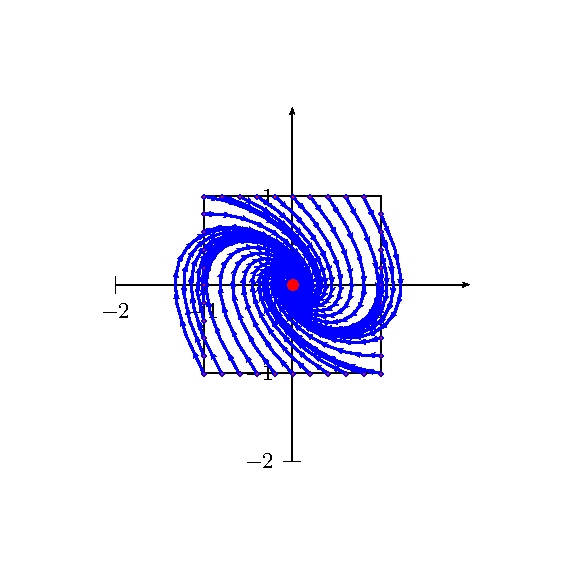
\includegraphics{stablePosition}
    \caption{Phase Plot of the Stable Posture}
    \label{fig:StablePosture}
  \end{center}
\end{figure}


Whereas the  posture in Figure~\ref{fig:ShipEqulibriumUnstable} is \emph{repelling} or \emph{unstable}, if being moved away from the equilibrium posture, the ship will move away further, as shown in Figure~\ref{fig:unStablePosture}.

\begin{figure}[!htbp]
  \begin{center}
      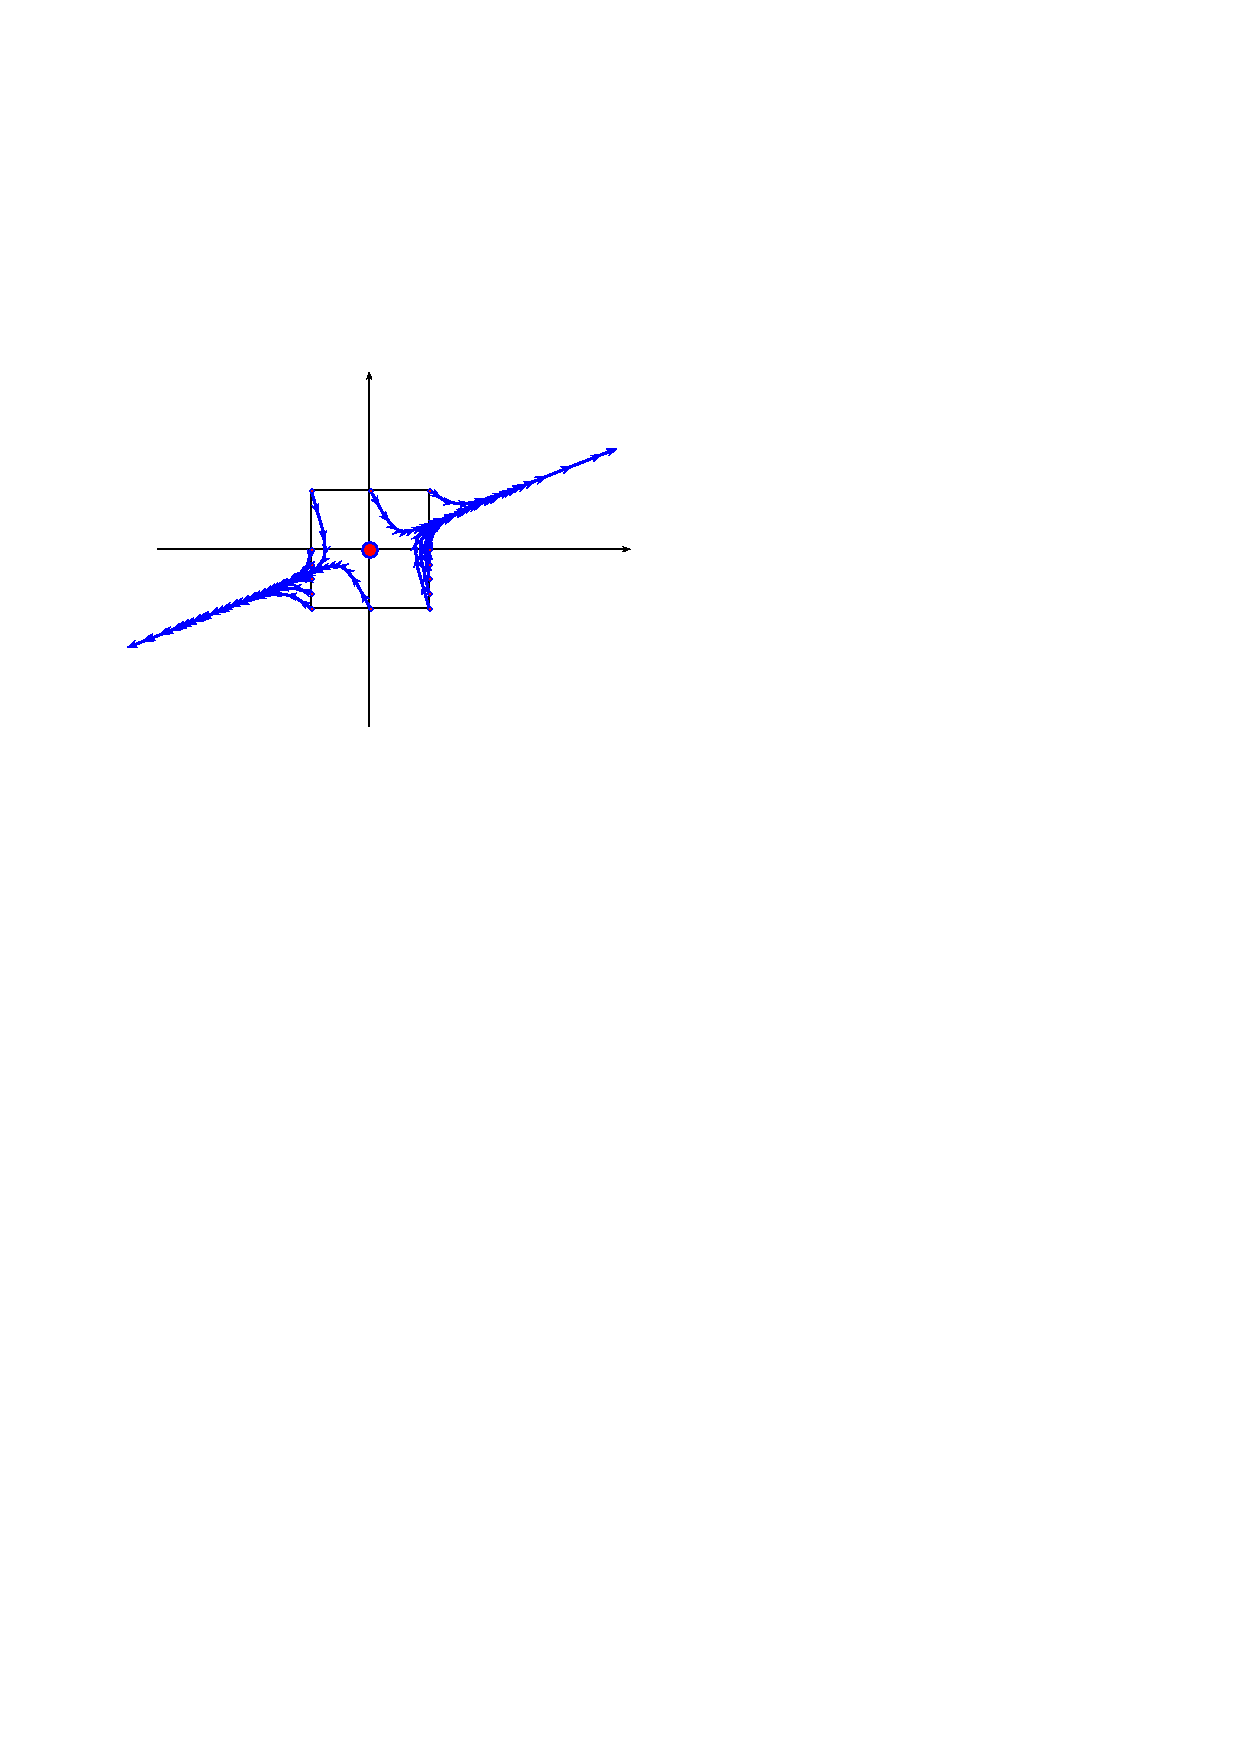
\includegraphics{unstablePosition}
    \caption{Phase Plot of the Unstable Posture}
    \label{fig:unStablePosture}
  \end{center}
\end{figure}


\subsubsection*{Trivial Task}
All the flows form the \emph{phase portrait} of the dynamic system. 
The discovery is that all the flows start from the repelling posture and ends at the attractive posture.
Several example curves are show in Figure ~\ref{fig:globalflow}.
This means no matter what the current posture is, the ship will return to the normal stable posture automatically.

This is an intrinsic property of the natural dynamics, and thanks to this, balancing is a trivial task which requires no control effort. 
This property is determined by the qualitative structure design criteria, makeing the centre of buoyancy  above the centre of gravity.

\begin{figure}[!htbp]
  \begin{center}
   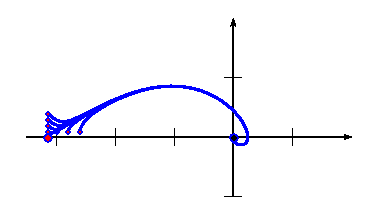
\includegraphics[width=0.7\textwidth]{ShipGlobalFlow}
   \caption{Global Properties of the Flows: All the curves start from the repelling posture(Red) and end at the attractive one(Blue)}
   \label{fig:globalflow}
  \end{center}
\end{figure}

 



\subsubsection*{Generalization of the Ship Example} 
This conclusion is independent of the shape, size, weight or material of the ship. 
In general cases, the same wave perturbation will result in different sway motions for different ships.
Howerver, as long as the qualitative structure design criteria is maintained, balancing remains ``easy''.
On phase portraits,  all the ships share following properties. 
\begin{itemize}
\item one repelling point 
\item one attractive point 
\item all flows start from repelling point and end at the  attractive point. 
\end{itemize}

In mathematical terms, all the phase portraits share the same topology structure of Figure~\ref{fig:topologyStructure}.

This phenomenon illustrates the principle idea of motion adaptation in \moit.
When the variations among individuals or situations result in motion variation, the qualitative dynamics or topological structure of the dynamic system remains invariant.

\begin{figure}[!htbp]
  \begin{center}
   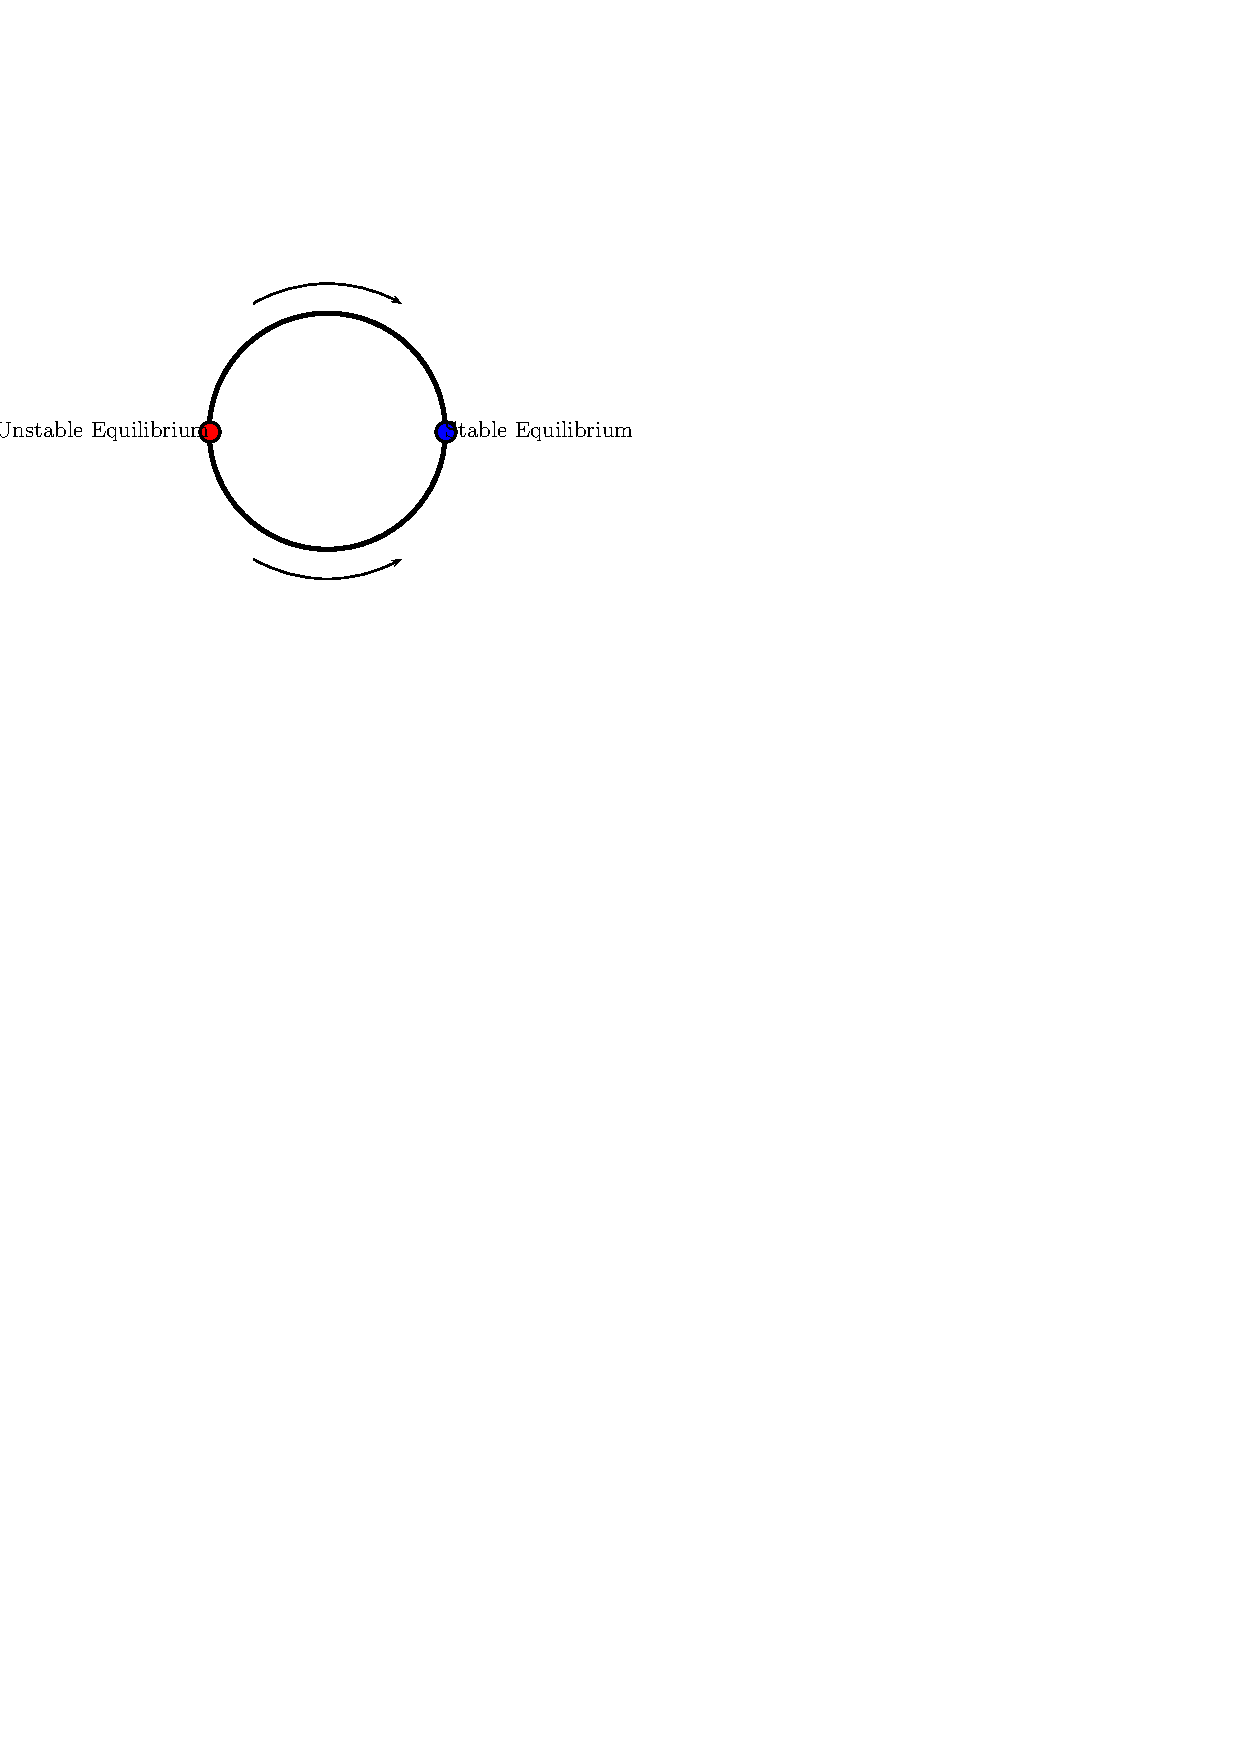
\includegraphics{topologyStructure}
   \caption{the topology  the phase portraits of ship dynamic}
   \label{fig:topologyStructure}
  \end{center}
\end{figure}




\subsection{The Mass Spring System:  Symmetry Transformation}
Despite the complexity of body structure, biological motor control is fast and accurate.
Such quantitative properties pose another puzzle in motor control research, as solving the complex dynamics directly would require prohibitive long computational time and excessive mental resources.

\moit proposes a new method to achieve the  speed and accuracy of motor control.
An efficient control strategy is based on the idea of transformation.
Without solving the dynamics, new motions are achieved through transforming template motions.
To keep the motion natural looking, control system chooses the transformation directions that are energy efficient, or in another term, allowed by the natural dynamics.


Such ideas can be illustrated by the following mass spring example, shown in Figure~\ref{fig:massspring}.
The mass spring system is selected for it captures some important properties of biological dynamics.
The compliant actuators of muscles work like springs, and rigid bones are modelled as mass.


\begin{figure}[!htbp]
  \begin{center}
    \includegraphics[width=0.7\textwidth]{MassSpring}
    \caption{the mass spring system}
    \label{fig:massspring}
  \end{center}
\end{figure}

\subsubsection*{Dynamics}
The canonical equation of mass spring system is
\begin{equation}
\label{eq:mass-spring}
\ddot{q}+q=0.
\end{equation}
where $q$ is the offset distance.

By defining the \emph{state variable}, $\state=[q,\qd]$, Equation~\ref{eq:mass-spring} can also be reformulated in the form as
\[
\dot{\state}=F(\state)
\]

 Figure~\ref{fig:massSpringPhasePlot} shows two flows passing through different states $x$ and $x'$ on the phase plot.


\begin{figure}[!htbp]
  \begin{center}
     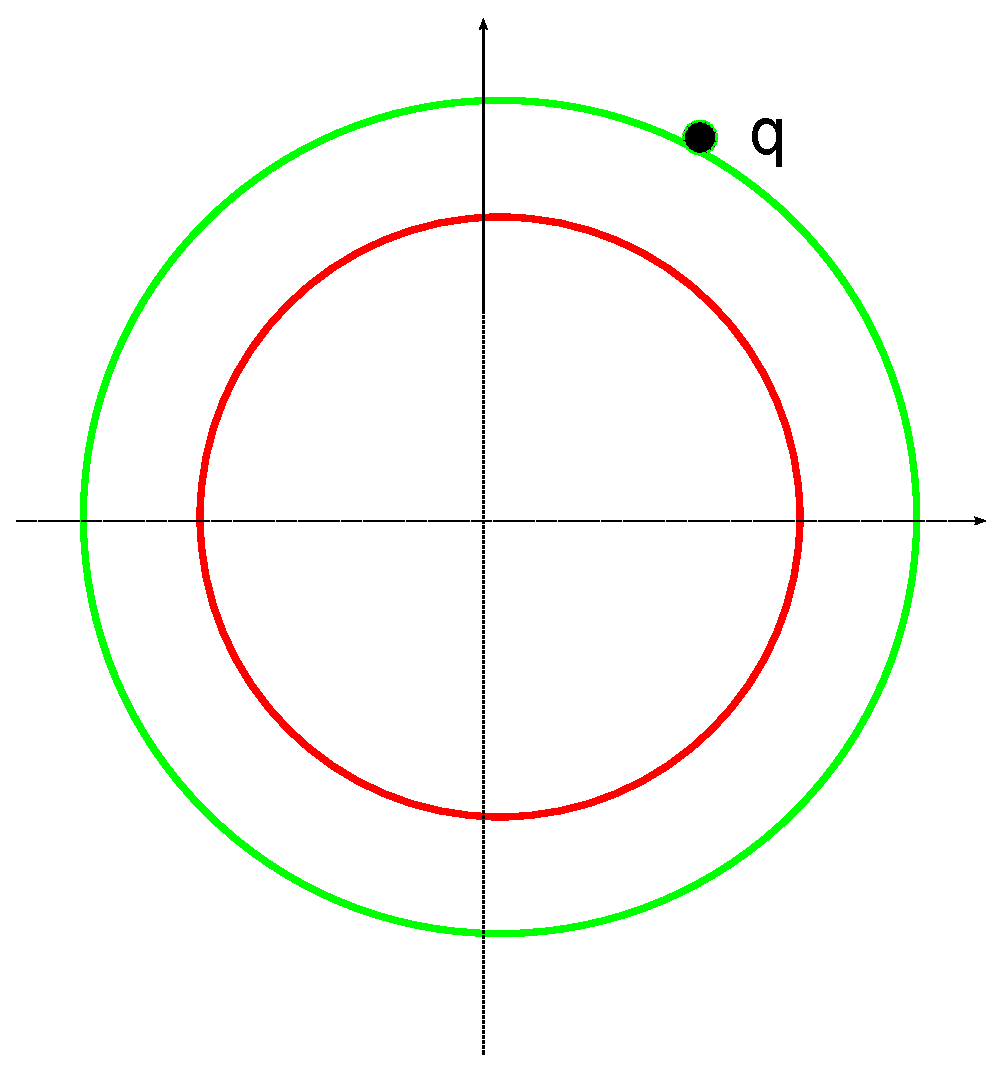
\includegraphics[width=0.5\textwidth]{MassSpringPhasePlot}
    \caption{Mass Spring Phase Plot:two motion curves are shown.The red one and the green pass through different states ($\state$ and $\state'$}
    \label{fig:massSpringPhasePlot}  
  \end{center}
\end{figure}

\subsubsection*{Symmetry and Transformation}
%It is highly unlikely animals can solve Equation~\ref{eq:mass-spring}.

The mass spring system has some ``symmetrical properties''.
Different flows share the same circle ``Shape''.
Without sovling the Equation~\ref{eq:mass-spring}, neew flows(solid ones) can be obtained by scaling the original(red) flow.

From a mechanical viewpoint, this is because the flows of mass spring system are energy preserving.
We can define the energy function
\[
E=\frac{1}{2}(m\qd^2+kq^2)
\]
where $k$ is the stiffness, $m$ is the mass.
When $m=1,k=1$, since $E$ is a constant, we can take $E=c$,
and obtain $q^2+\qd^2=2c$, which is the implicit function of a circle.

Therefore, given the template flows that pass through  $\state$, for the state $\state'$, by checking the energy, the scale transformation from red to green can be worked out.
In this manner, we botained the future motion after $\state'$, without sovling the dynamics.


\subsubsection*{Dynamic Perception and Local Motor Invariant}

The idea ``transformation and symmetry'' may shed light on dynamic perception. 
It is highly unlikely animals can solve Equation~\ref{eq:mass-spring} to understand mass spring system.
As an alternative, the dynamics can be encoded in a different manner: a motion template and the symmetry property. 
If so, observed motions can be validated by being checked against motion templates in our memory.

To make it better, it is even unnecessary to working out the transformation, it is enough just to check some property invariant under transformation.
For the mass spring system example, we can check the “shape” of the flow, or from a mechanical perspective, check the energy preserving property.

 
The invariant properties like energy preserving or shape can be quantitative measured, they are invariant only when system flows move in a specific direction, thus are called  \emph{Local Motor Invariant}. 


\section{Contribution}

Compared with current \cms methods, the new approach has several advantages:
\begin{enumerate}
\HiItem {More Types of Adaptation}
Most dynamic methods only focus on generating responsive motion to dynamic perturbation.
Adaptations across different characters are solved with a different method and treated as a independent research topic(motion re-targeting).
\moit unifies different  adaptations in one theory.
The mathematical idea of topology conjugacy  incorporates both motion re-targeting and  perturbation responses  in an unified framework.
Thus \moit can generate more types of adaptation.
\HiItem {Better Usability}.
For many \cms methods, each \dof ~is controlled independently.
When modifying motions, animator has to modify each \dof, which is tedious work.

In \moit, adaptation is achieved by applying transformation.
Each transformation can be parameterized by one parameter. 
By specify only one parameter for the transformation, control inputs of all {\dof}s are modified automatically, which is more easy to use.

\HiItem {No Reference Motion Needed}
\moit relies on the dynamics of body and environment.
Motion Capture Data is not needed as reference input.
In situations, this method can generate new motion that can not be captured.


\HiItem {Computationally Efficient} 
This motion synthesis approach requires little computation time and memory, it suits real-time applications.
\HiItem {Dynamic Motion Transition}
Dynamic motion transition is developed upon solid theory foundation.

\end{enumerate}

Because of its biological foundation,
algorithms and simulation results of \moit  might shed light into biology research.
Some conclusion and control techniques can be treated as candidate theory that needs further verification.

\begin{enumerate}
\item 
Motion Primitive is an old idea in biological research, but there is no agreement on the definition and underlying reason.
Biological research has tried to identify motion primitive by exploring the neural anatomy, EMG signal or muscle activation pattern.

\moit  explains the motion primitive from dynamic viewpoint.
This theory is more complete.
Besides identification, it also answers why certain motions are primitives and others are not,
how many motion primitives we have,  and where they come from.

\item One supporting theory of motion primitive is the muscle synergy:
Generating motion by actuating muscles, muscles are not controlled independently but worked in group. 
Many research in synergy by empirical methods. 

In \moit, when control is applied to ensure transformation, actuators are controlled in an ``synergy manner''.
\moit provides a candidate  ``synergy'' method for muscle control.

\item For the neural structure \emph{Central Pattern Generator}(\cpg) , their roles in motor control are well agreed.
While detail strategy for adjust \cpg parameters according to motor purpose is still lacking.
The \moit provides an theory for modifying the \cpg parameters with mathematical rigidity.


\item  Motion and dynamic perception mechanism of neural system is still unclear.
The motor invariant theory proposes a computationally efficient mathematical machinery.
\end{enumerate}







\section{Organization of the Thesis}

This thesis is organized as follows.
 
In Chapter~\ref{chap:background}, previous research on motion synthesis and biological motor control are discussed, which are the motivation and justification of \moit.
 
In Chapter~\ref{chap:gi}, \emph{Qualitative Dynamicss} is introduced to explain motion primitives. 
Biological based  methods for maintaining the global motor invariant are developed.

Chapter~\ref{chap:li} focuses on the idea of Local Motor Invariant and Symmetry.
Lie Group theory is  introduced  to analyse the symmetry properties in motion dynamics.
Symmetry Controllers are developed for adaptation motions.
 


Chapter~\ref{chap:msf} discusses the combination problems.
For each motion primitive,  strategies are developed to preserve global and local motor invariant simultaneously.
Motion primitive transition is discussed and methods for combining motion elements into more complex motion is discussed.
As an animation system, the software architecture and work flow are discussed at the end.

Chapter~\ref{chap:gi},~\ref{chap:li},~\ref{chap:msf} lay the theoretical foundation of \moit.
Following chapters focus on application in \cms.



Chapter~\ref{chap:walk} focuses the tweaking of one primitive.
Bipedal walking is chosen, which is one of the most challenging problem for current \cms research.
Motor Invariant Theory introduces a method to boost the stability and generate adaptive gaits.


In Chapter~\ref{chap:stance}, combinations of motion primitives are discussed.
A new balancing motion primitive is developed. 
Transitional motions are generated for stance to walk and walk to stance transitions.

In Chapter~\ref{chap:highdor}, extensions of motor invariant theory to more complex characters are discussed.
Three strategies are developed to simplify the problem for different situations.

This thesis ended with Chapter~\ref{chap:con}. 
After discussion of new finding of this research, some new questions and ideas for graphics and neural science are proposed for further research .





%%% ----------------------------------------------------------------------


%%% Local Variables: 
%%% mode: latex
%%% TeX-master: "../thesis"
%%% End: 


% \pagebreak[4]
% \hspace*{1cm}
% \pagebreak[4]
% \hspace*{1cm}
% \pagebreak[4]

\chapter{My First Chapter But Note The Numbering ...}
\ifpdf
    \graphicspath{{Chapter1/Chapter1Figs/PNG/}{Chapter1/Chapter1Figs/PDF/}{Chapter1/Chapter1Figs/}}
\else
    \graphicspath{{Chapter1/Chapter1Figs/EPS/}{Chapter1/Chapter1Figs/}}
\fi

\section{First Paragraph}
And now I begin my first chapter here ...

Here is an equation\footnote{the notation is explained in the nomenclature section :-)}:
\begin{eqnarray}
CIF: \hspace*{5mm}F_0^j(a) &=& \frac{1}{2\pi \iota} \oint_{\gamma} \frac{F_0^j(z)}{z - a} dz
\end{eqnarray}
\nomenclature[zcif]{$CIF$}{Cauchy's Integral Formula}                                % first letter Z is for Acronyms 
\nomenclature[aF]{$F$}{complex function}                                                   % first letter A is for Roman symbols
\nomenclature[gp]{$\pi$}{ $\simeq 3.14\ldots$}                                             % first letter G is for Greek Symbols
\nomenclature[gi]{$\iota$}{unit imaginary number $\sqrt{-1}$}                      % first letter G is for Greek Symbols
\nomenclature[gg]{$\gamma$}{a simply closed curve on a complex plane}  % first letter G is for Greek Symbols
\nomenclature[xi]{$\oint_\gamma$}{integration around a curve $\gamma$} % first letter X is for Other Symbols
\nomenclature[rj]{$j$}{superscript index}                                                       % first letter R is for superscripts
\nomenclature[s0]{$0$}{subscript index}                                                        % first letter S is for subscripts

\section{Second Paragraph}
and here I write more ...\cite{texbook}

\subsection{sub first paragraph}
... and some more ...

Now I would like to cite the following: \cite{latex} and \cite{texbook}
and \cite{Rud73}.

I would also like to include a picture ...

\begin{figure}[!htbp]
  \begin{center}
    \leavevmode
    \ifpdf
      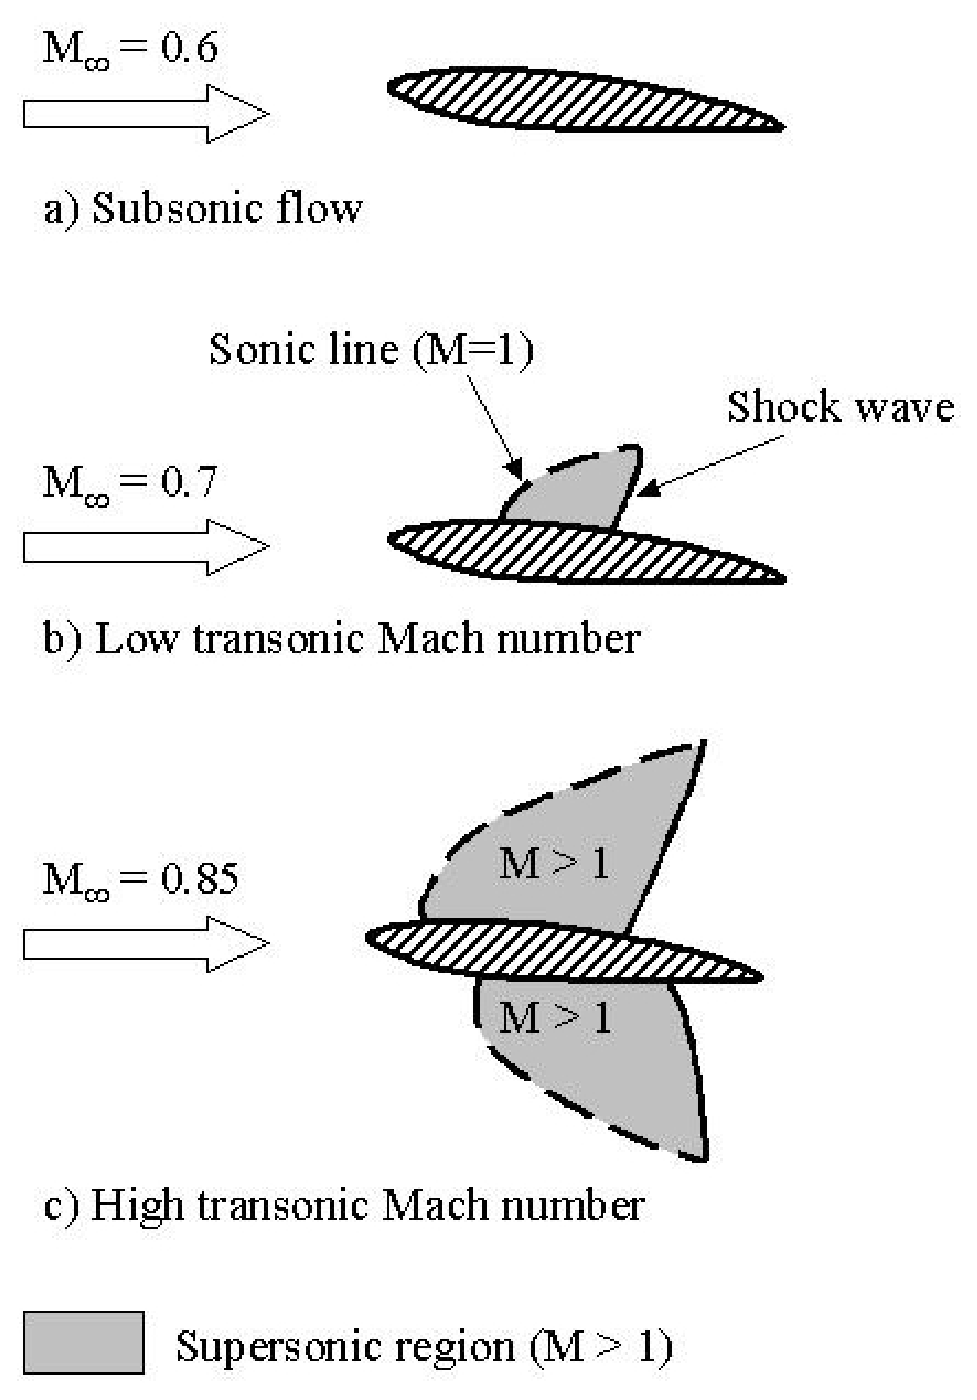
\includegraphics[height=6in]{aflow}
    \else
      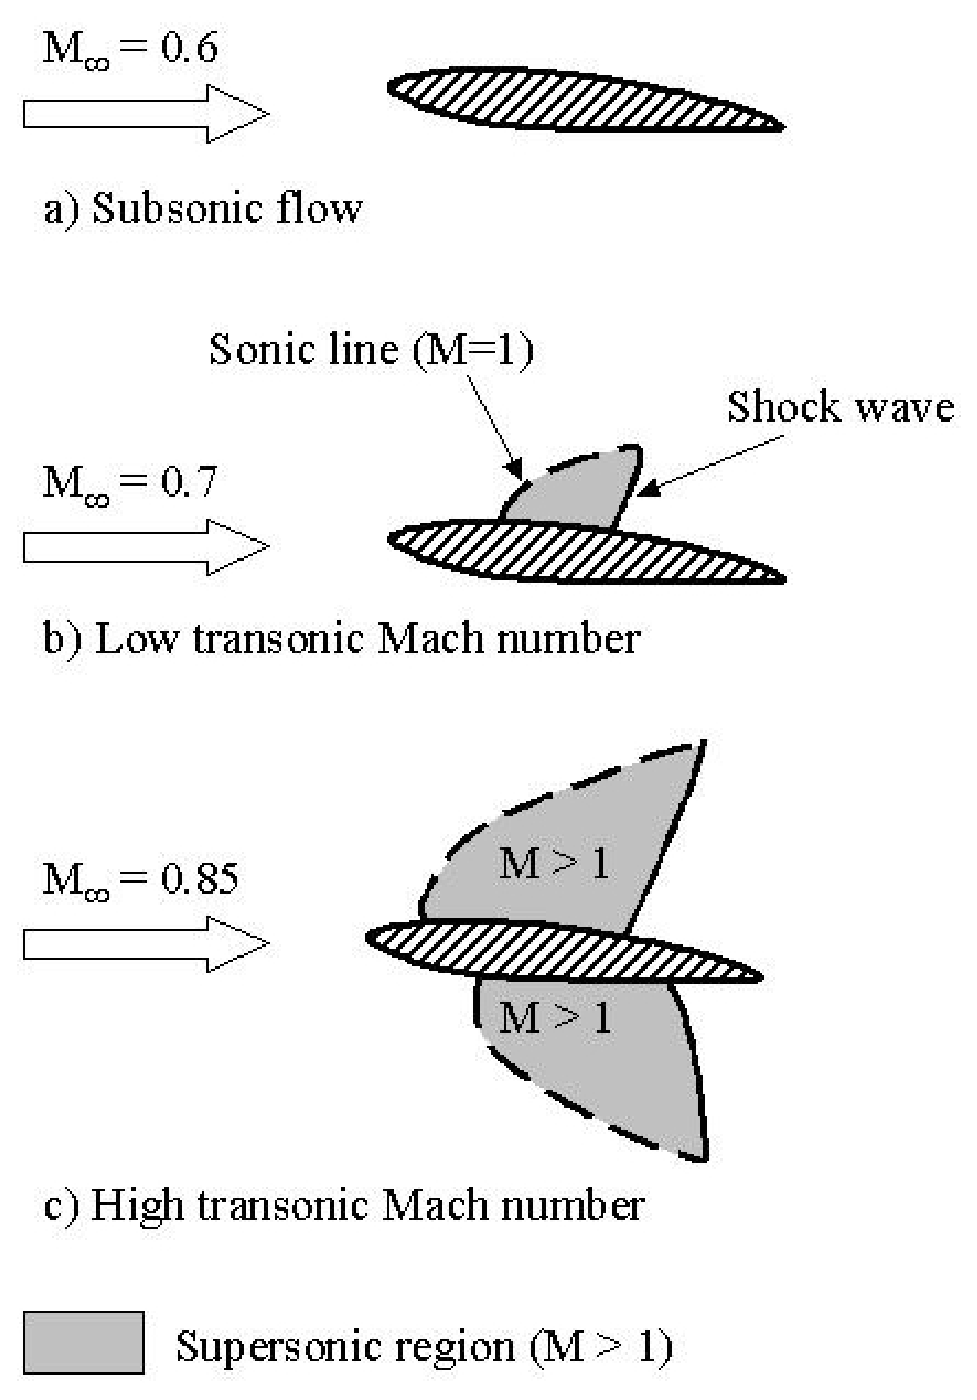
\includegraphics[bb = 92 86 545 742, height=6in]{aflow}
    \fi
    \caption{Airfoil Picture}
    \label{FigAir}
  \end{center}
\end{figure}

% above code has been macro-fied in Classes/MacroFile.tex file
%\InsertFig{\IncludeGraphicsH{aflow}{6in}{92 86 545 742}}{Airfoil Picture}{FigAir}

So as we have now labelled it we can reference it, like so (\ref{FigAir}) and it
is on Page \pageref{FigAir}. And as we can see, it is a very nice picture and we
can talk about it all we want and when we are tired we can move on to the next
chapter ...

I would also like to add an extra bookmark in acroread like so ...
\ifpdf
  \pdfbookmark[2]{bookmark text is here}{And this is what I want bookmarked}
\fi
% ------------------------------------------------------------------------


%%% Local Variables: 
%%% mode: latex
%%% TeX-master: "../thesis"
%%% End: 

\chapter{My Second Chapter}
\ifpdf
    \graphicspath{{Chapter2/Chapter2Figs/PNG/}{Chapter2/Chapter2Figs/PDF/}{Chapter2/Chapter2Figs/}}
\else
    \graphicspath{{Chapter2/Chapter2Figs/EPS/}{Chapter2/Chapter2Figs/}}
\fi

\section{First Section}
\markboth{\MakeUppercase{\thechapter. My Second Chapter }}
And now I begin my second chapter here ...

\section{Second Section}
\markboth{\MakeUppercase{\thechapter. My Second Chapter }}
and here I write more ...

\subsection{first subsection in the Second Section}
... and some more ...

\subsection{second subsection in the Second Section}
... and some more ...

\subsection{third subsection in the Second Section}
... and some more ...

% ------------------------------------------------------------------------

%%% Local Variables: 
%%% mode: latex
%%% TeX-master: "../thesis"
%%% End: 

\chapter{My Third Chapter}
\ifpdf
    \graphicspath{{Chapter3/Chapter3Figs/PNG/}{Chapter3/Chapter3Figs/PDF/}{Chapter3/Chapter3Figs/}}
\else
    \graphicspath{{Chapter3/Chapter3Figs/EPS/}{Chapter3/Chapter3Figs/}}
\fi

\section{First Section of the Third Chapter}
\markboth{\MakeUppercase{\thechapter. My Third Chapter }}{\thechapter. My Third Chapter}
And now I begin my third chapter here ...

\subsection{first subsection in the First Section}
... and some more 

\subsection{second subsection in the First Section}
... and some more ...

\subsubsection{first subsub section in the second subsection}
... and some more in the first subsub section otherwise it all looks the same
doesn't it? well we can add some text to it ...

\subsection{third subsection in the First Section}
... and some more ...

\subsubsection{first subsub section in the third subsection}
... and some more in the first subsub section otherwise it all looks the same
doesn't it? well we can add some text to it and some more and some more and
some more and some more and some more and some more and some more ...

\subsubsection{second subsub section in the third subsection}
... and some more in the first subsub section otherwise it all looks the same
doesn't it? well we can add some text to it ...

\section{Second Section of the Third Chapter}
\markboth{\MakeUppercase{\thechapter. My Third Chapter }}{\thechapter. My Third Chapter}
and here I write more ...

% ------------------------------------------------------------------------


%%% Local Variables: 
%%% mode: latex
%%% TeX-master: "../thesis"
%%% End: 

\def\baselinestretch{1}
\chapter{CONCLUSION AND FURTHER WORK}
\label{chap:con}
\graphicspath{{Conclusions/ConclusionsFigs/EPS/}{Conclusions/ConclusionsFigs/}}


\def\baselinestretch{1.66}

\section{Conclusion}

Inspired by the biological research and robotic engineering experiments, in this thesis, a new theory, the motor invariant theory, of motor control is established.
In the \moit, the hypothesis is that animals explore the natural dynamics as the basis for synthesizing motion.
The mathematical reason is because of the special properties of natural dynamics.
The evolution of the body and environment forms some stable attractors in the dynamics, which provides the stability necessary for motion.
To adapt motion, animals modify the system dynamics in a specific way, the modify the modify many properties of the attractor, but not the stability.
New mathematical tools is introduced for modelling this idea, the topology conjugacy.
Under this mathematical framework, many old ideas of biological motor control can be unified.


This theory is a contribution to the biological motor control research.
They provides a clear mathematical meaning for  motion primitive hypothesis.
It answers the question why motions are so similar but varies so much.
In the \moit theory, the biological control is not based following the trajectory,
but modifying the system properties to form attractors.
In an certain environment and body dynamic property,
the ways to form attractors is limited.
thus result in the limited number of motion primitives and stereotype patterns for many motion tasks.



The new idea of motor dynamics provides a valuable alternative for motion synthesis paradigm.
If motor control is based on utilizing the natural dynamics and involves little reasoning effort.
For the computer animation research, complex trajectory planning and expensive inverse dynamic computation of current motion synthesis method can be get rid of,  motion synthesis almost as efficient as forward dynamic simulation.
To this end, neural oscillating entrainment and lie group control actions are introduced, the two methods modifies the motions qualitatively and quantitatively.
Entrainment  models the biological center pattern generator, which exists in the spine cord in many vertebrate.
While idea of lie group action close related to the vision system, maybe a model for control effects of vision system.
A new hierarchy in control framework is established.
The low level controller(\cpg) maintain the stability or qualitative property.
While high level controller(the vision cortex) control the precision or quantitative properties of motion.
The new method has been applied to some typical motions, including walking, standing and swimming.
Adaptive and natural looking results are achieved with very low computational cost.
Compared with tradition methods, the new method is more easy to set-up and has fewer parameters in adapting motion.


The dynamic perspective may provides impactive insights in two many fields close related to motor control.
An simple example is it may provided a different understanding of the evolution of motion, body structural and environment.
Also the new insights of motor control close related to motion perception.
Nature provides many insightful ideas, but lots questions remained to be answered.













 




\section{Further Work}
Motor Invariant Theory is not an improvement of already \cms techniques, it is a different paradigms.
Research in this thesis does explore the full implication and potential of new born theory.
For a new born theory, there are rooms to improvement, new techniques and even new questions.
In this section, we discuss several potential topics that may interest computer graphic community or biological research.

\subsection{Stable Templates Of Motion Primitives}

Research in this thesis starts from unstable system,  stability are enhanced by adding control effort.
Motor control is a complex task, in many cases, it is impossible to model all the control efforts that turn an unstable system into stable ones.


A alternative method is start from a stable system and modify its shape to match the observation.
Such methods may lost the details of motion but provides better stability and controllability. 
For games or film production, this idea may be important, animator requires controllability and stability over physical realistic.
For characters performance acrobat, the characters must not fall even dynamic system is unstable in nature.




\subsection{More Type Of Symmetry}
More type of symmetry will generate more type of transformation that can be applied  to the adapt motion.
All the group actions adopted in this research are linear transformation group, which are easy to compute.
But the types of transformation is very limited.
Exploring more types of symmetry may provides a different adaptation schemes and may expand the theory to different motion primitives.
\begin{itemize}

\HiItem{Discrete Symmetry Properties}
Bipedal motions are synthesized in this research, an interesting idea is whether four or more legs motions can be built based on the bipedal walking strategy.

This can be done by exploring another type of symmetry: discrete symmetry.
For the house hound, the hind leg and font leg will move in synchronize or in antiphase.




\HiItem{Non-linear Symmetry from Structural Parameter Turning}
Non-linear symmetry preserving transformation will generate more type of adaptation.
Since non-linear transformation are more difficult to find, it remains questionable how the biological system perceive it and apply it for motion adaptation.
But non-linear transformation is suitable for modelling the transformation  results from tweaking system parameters.
For the idea of structural stability we know the results of tweaking system parameters is equivalent to have a one one mapping transformation.
Further research result from non-linear transformation may potentially completely solved the motion re-targeting problem 


\HiItem{Symmetry of Partial Differential System}

All the methods developed are for  ordinary differential equations, which is good enough for rigid body dynamics.
In fact the topological property and symmetrical property also applies to partial differential equations.
For example of Lorenz transformation group and Maxwell equation.

Symmetrical of partial differential equations are important for they may extend the control strategy  to control the motion elastic body or locomotion in fluid.
Such motion are more expensive are little addressed by current \cms methods.


\end{itemize}

To exploring more types of symmetry, reformulation the form of equations may ease the task.
Current dynamic equations are based a fix coordinates frame.
It is helpful to formulate the equations in the coordinate free manner or in the local frame.






\subsection{Transform the Motion Capture Data}
For computer animation, even methods for simulation high dimensional characters are proposed.
It may be impractical to synthesize all types of motions by procedure method.
An alternative method is use dynamic simulation to modify motion capture data, which is well addressed in many research in computer graphic community.



Based on the idea of topological equivalence, 
motion primitive of different persons or motions of different situation should have the property of topological equivalent.
In state space, there should exist a one to one mapping transformation function.
Motion Data can be transformed into the state space and apply transformation.


We can use the low dimensional model to find the one to one mapping relationship, 
which are applied to transform the high dimensional motion capture data.
Potentially, this method may retain the motion details and involves little computational work. 





\subsection{Muscle Actuation}
In the thesis, control effort are applied directly to each \dof of the mechanical system.
In biological research, this process is not so direct.
Neural system generate some chemicals which affects the material properties of muscles.
Force are generated as an indirect side effects.


The question muscle actuation is untouched in this research,
but with a second thought, \moit also provides an alternative idea of muscle action.
Transformation is the reason for applying control effort,
the actuation of muscles can be calculated directly from the transformation, without caring about the force generated.
From this perspective, muscle actuation can be more easy than calculating the forces.


For the simple  mass spring system.
offset can implemented by changing the rest length parameter $d$.
Speed action can be implemented by changing the stiffness $K$.
and energy scaling can be achieved by adjust the stiffness $K$ and then restore it.
 

The reason is transformation can be achieved by two methods.
Either control effort or by changing the system parameters.

For biological system, the changing parameters method may be better for it will help motor control system get rid of the necessary feedback and computation. 
In fact most of control effort in the thesis are potential shaping, which only involves of modify the potential energy.
If muscles are modelled as spring, then potential energy shaping can also achieved through modifying spring parameters.

The complex muscle structure may provide a mechanism for fine turning the deformation of the phase portrait and make the attractor into any possible shape.
This idea may propose an conjecture for further biological research.
For graphic research, incorporating muscles in this manner will have no effects on motion synthesis or computational work.
The potential benefits is that the parameters of muscles can effect the skin deformation.



\subsection{Perception based Dynamics}
Motion perception is an high level capacity, it is based up our object recognition ability and our dynamic reasoning ability.
And many the physiological questions in computer graphics may finally conclude with the recognition and perception research in neural science.
The introduction of a motion synthesis method also touch the question of dynamic motion perception and encoding problem in intelligence.
The topological equivalence and symmetry may also provides an understanding of the perception problem.

Based on the idea of topology equivalence,
Neural system may not need to encode the details of dynamic system, neural system can form an analogous dynamic system in our brain that is analogy to the real dynamics.
Such model will lack the details accuracy, but get the qualitative properties right.

Based on the idea of symmetry,
Neural system may store some experience and the symmetrical property of dynamics in memory.
The dynamics validity by transform our experience to match observation.


We are not still not sure which method is better, but both of methods are more practical for the neural system than forming a symbolic equation solving the differential equations numerically in our brain.
Maybe a new dynamic simulator can be designed to test this hypothesis.
Dynamic simulator can be build upon the topology and the symmetry property.
Animator can specify animation by specify its attractor and the transformation being  applied.
If the hypothesis is true, even the method will generate physically inaccurate results, audience will not notice it.

\subsection{Rethink about the uncanny valley}
In \cms research, uncanny valley is a challenging phenomenon of perception at the  central. 
When the characters  becomes more and more realistic, there is a big drop in the perception of likeness.
Only over the valley, perception likeness start to increase;
At currently, little is known about overcoming the phenomenon.
mainly because the mechanism behind such phenomenon is unclear.

At the end of the the thesis, a conjecture is proposed by extending the idea of motor invariant theory.
Figure~\ref{fig:uncannyValley}.

\begin{figure}[!htbp]
  \begin{center}
      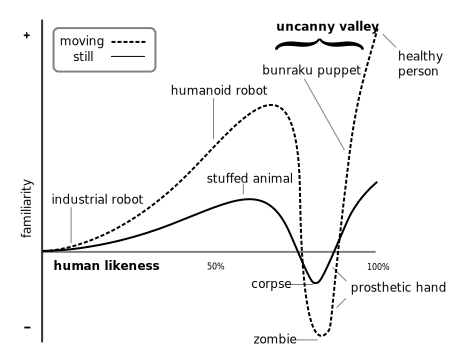
\includegraphics[width=0.5\textwidth]{Mori_Uncanny_Valley}
    \caption{Uncanny Valley}
    \label{fig:uncannyValley}
\end{center}
\end{figure}

The reason behind the uncanny valley is a  a switch of perception mechanism.
For the unfamiliar, the perception mechanism is based on analogy,
where the the identification of qualitative properties plays the major role.
As long as the qualitative properties is the the same with our experience, we may accept characters as ``believable''.
In this situation we are checking the Global Motor Invariant.

When the object becomes more familiar, it will trigger our experience memory.
Details are utilized to check the observation against memory,
which closely relate to the idea of Local Motor Invariant.


A object that have desired qualitative property may not have the quantitative details for quantitative perception mechanism.
When the switch of mechanism results in a drop in likeness.
This proposal is bold and early, but might be a worthwhile topic for further biological and physiological research.





%%% ----------------------------------------------------------------------

% ------------------------------------------------------------------------

%%% Local Variables: 
%%% mode: latex
%%% TeX-master: "../thesis"
%%% End: 


\backmatter % book mode only
\appendix
\chapter{Appdx A:Dynamic Equation for Passive Walking}

\section{Knee Free Phase}

\[
M(q)\ddot{q}+C(q,\dot{q})\dot{q}+N=\tau\]


\[
M(q)=\left[\begin{array}{ccc}
M_{11} & M_{12} & M_{13}\\
M_{12} & M_{22} & M_{23}\\
M_{13} & M_{23} & M_{33}\end{array}\right]
\]

\[
M_{11}=m_{s}^{st}a_{1}^{2}+m_{t}^{st}(l_{s}+a_{2})^{2}+(m_{h}+m_{t}^{sw}+m_{s}^{sw})L^{2}\]


\[
M_{12}=-(m_{t}^{sw}b_{2}+m_{s}^{sw}l_{t})Lcos(q_{2}-q_{1})\]


\[
M_{13}=-m_{s}^{sw}b_{1}cos(q_{3}-q_{1})\]


\[
M_{22}=m_{t}^{sw}b_{2}^{2}+m_{s}^{sw}l_{t}^{2}\]
\[
M_{23}=m_{s}^{sw}l_{t}b_{1}cos(q_{3}-q_{2})\]


\[
M_{33}=m_{s}^{sw}b_{1}^{2}\]


\[
C(q,\dot{q})=\left[\begin{array}{ccc}
0 & C_{12}\dot{q_{2}} & C_{13}\dot{q}_{3}\\
-C_{12}\dot{q}_{1} & 0 & C_{23}\dot{q}_{3}\\
-C_{13}\dot{q_{1}} & -C_{23}\dot{q}_{2} & 0\end{array}\right]\]


\[
C_{12}=-(m_{t}^{sw}b_{2}+m_{s}^{sw}l_{t})Lsin(q_{1}-q_{2})\]


\[
C_{13}=-m_{s}^{sw}b_{1}Lsin(q_{1}-q_{3})\]


\[
C_{23}=m_{s}^{sw}l_{t}b_{1}sin(q_{3}-q_{2})\]



\[
N=\left[\begin{array}{c}
-(m_{s}^{st}a_{1}+m_{t}^{st}(l_{s}+a_{2})+(m_{h}+m_{s}^{sw}+m_{t}^{sw})L)g\mathbf{\mathrm{sin}}(q_{1})\\
(m_{t}^{sw}b_{2}+m_{s}^{sw}l_{t})gsin(q_{2})\\
m_{s}^{sw}b_{1}gsin(q_{3})\end{array}\right]\]


\section{Knee Strike}

\[
Q^{+}\left[\begin{array}{c}
\dot{q}_{1}\\
\dot{q}_{2}\end{array}\right]^{+}=Q^{-}\left[\begin{array}{c}
\dot{q}_{1}\\
\dot{q}_{2}\\
\dot{q}_{3}\end{array}\right]^{-}\]


\[
q_{3}^{+}=q_{2}^{+}\]


\[
Q^{-}=\left[\begin{array}{ccc}
Q_{11}^{-} & Q_{12}^{-} & Q_{13}^{-}\\
Q_{21}^{-} & Q_{22}^{-} & Q_{23}^{-}\end{array}\right]\]


\[
Q^{+}=\left[\begin{array}{cc}
Q_{11}^{+} & Q_{12}^{+}\\
Q_{21}^{+} & Q_{22}^{+}\end{array}\right]\]


\[
Q_{11}^{-}=-(m_{s}^{sw}l_{t}+m_{t}^{sw}b_{2})Lcos(q_{1}-q_{2})-m_{s}^{sw}b_{1}cos(q_{1}-q_{3})+(m_{t}^{sw}+m_{s}^{sw}+m_{h})L^{2}+m_{s}^{st}a_{1}^{2}+m_{t}^{st}(l_{s}+a_{2})^{2}\]


\[
Q_{12}^{-}=-(m_{s}^{sw}l_{s}+m_{t}^{sw})Lcos(q_{1}-q_{2})+m_{s}^{sw}b_{1}l_{t}cos(q_{2}-q_{3})+m_{t}^{sw}b_{2}^{2}+m_{s}^{sw}l_{t}^{2}\]


\[
Q_{13}^{-}=-m_{s}^{sw}b_{1}Lcos(q_{1}-q_{3})+m_{s}^{sw}b_{1}l_{t}cos(q_{2}-q_{3})+m_{s}^{sw}b_{1}b_{2}\]


\[
Q_{21}^{-}=-(m_{s}^{sw}l_{t}+m_{t}^{sw}b_{2})Lcos(q_{1}-q_{2})-m_{s}^{sw}b_{1}Lcos(q_{1}-q_{3})\]


\[
Q_{22}^{-}=m_{s}^{sw}b_{1}l_{t}cos(q_{2}-q_{3})+m_{s}^{sw}l_{t}^{2}+m_{t}^{sw}b_{2}^{2}\]
\[
Q_{23}^{-}=m_{s}^{sw}b_{1}l_{t}cos(q_{2}-q_{3})+m_{s}^{sw}b_{1}^{2}\]


\[
Q_{11}^{+}=Q_{21}^{+}+m_{t}^{st}(l_{s}+a_{2})^{2}+(m_{h}+m_{t}^{sw}+m_{s}^{sw})L^{2}+m_{s}^{st}a_{1}^{2}\]


\[
Q_{12}^{+}=Q_{21}^{+}+m_{s}^{sw}(l_{t}+b_{1})^{2}+m_{t}^{sw}b_{2}^{2}\]


\[
Q_{21}^{+}=-(m_{s}^{sw}(b_{1}+l_{t})+m_{t}^{sw}b_{2})Lcos(q_{1}-q_{2})\]


\[
Q_{22}^{+}=m_{s}^{sw}(b_{1}+l_{t})^{2}+m_{t}^{sw}b_{2}^{2}\]



\section{Knee Lock Phase}


\[
M(q)\ddot{q}+C(q,\dot{q})\dot{q}+N=\tau\]


\[M(q)=\left[\begin{array}{cc}
M_{11} & M_{12}\\
M_{12} & M_{22}\end{array}\right]
\]

\[
M_{11}=m_{s}^{st}a_{1}^{2}+m_{t}^{st}(l_{s}+a_{2})^{2}+(m_{h}+m_{t}^{sw}+m_{s}^{sw})L^{2}\]


\[
M_{12}=-(m_{t}^{sw}b_{2}+m_{s}(l_{t}+b_{1}))Lcos(q_{2}-q_{1})\]


\[
C(q,\dot{q})=\left[\begin{array}{cc}
0 & C_{12}\dot{q}_{2}\\
-C_{12}\dot{q}_{1} & 0\end{array}\right]
\]

\[
C_{12}=(m_{t}^{sw}b_{2}+m_{s}(l_{t}+b_{1}))Lsin(q_{1}-q_{2})
\]

\[
N=\left[\begin{array}{c}
-(m_{s}^{st}a_{1}+m_{t}^{st}(l_{s}+a_{2})+(m_{h}+m_{s}^{sw}+m_{t}^{sw})L)g\mathbf{\mathrm{sin}}(q_{1})\\
(m_{t}^{sw}b_{2}+m_{s}^{sw}(l_{t}+b_{1}))gsin(q_{2})\end{array}\right]
\]

\section{Heel Strike Phase}

\[
Q^{+}\dot{q}^{+}=Q^{-}\dot{q}^{-}\]



\[
q^{+}=\left[\begin{array}{cc}
0 & 1\\
1 & 0\\
1 & 0\end{array}\right]q^{-}\]




\[
\dot{q}_{3}^{+}=\dot{q}_{2}^{+}\]


\[
Q^{-}=\left[\begin{array}{cc}
Q_{11}^{-} & Q_{22}^{-}\\
Q_{21}^{-} & 0\end{array}\right]\]


\[
Q_{11}^{-}=Q_{21}^{-}+(m_{h}L+m_{t}^{st}(a_{2}+l_{s})+m_{s}^{st}a_{1}+m_{t}^{sw}(a_{2}+l_{s})+m_{s}a_{1})Lcos(q_{1}-q_{2})\]


\[
Q_{12}^{-}=-m_{s}^{sw}a_{1}(l_{t}+b_{1})-m_{t}^{sw}b_{2}(l_{s}+a_{2})\]


\[
Q_{21}^{-}=-m_{s}^{st}a_{1}(l_{t}+b_{1})-m_{t}^{st}b_{2}(l_{s}+a_{2})\]



\[
Q_{11}^{+}=Q_{21}^{+}+(m_{s}^{st}+m_{t}^{st}+m_{h})L^{2}+m_{s}^{sw}a_{1}^{2}+m_{t}^{sw}(a_{2}+l_{s})^{2}\]


\[
Q_{12}^{+}=Q_{21}^{+}+(m_{s}^{st}+m_{t}^{st}+m_{h})L^{2}+m_{s}^{sw}a_{1}^{2}+m_{t}^{sw}(a_{2}+l_{s})^{2}\]


\[
Q_{21}^{+}=-(m_{s}^{st}(b_{1}+l_{t})+m_{t}^{st}b_{2})Lcos(q_{1}-q_{2})\]


\[
Q_{22}^{+}=m_{s}^{st}(l_{t}+b_{1})^{2}+m_{t}^{st}b_{2}^{2}\]






% ------------------------------------------------------------------------

%%% Local Variables: 
%%% mode: latex
%%% TeX-master: "../thesis"
%%% End: 

\chapter{Appdx B}

and here I put some more postamble ...

% ------------------------------------------------------------------------

%%% Local Variables: 
%%% mode: latex
%%% TeX-master: "../thesis"
%%% End: 



%new
%\bibliographystyle{plainnat}
%endnew
\bibliographystyle{Classes/CUEDbiblio}
%\bibliographystyle{Classes/jmb}
%\bibliographystyle{plainnat} %this works with package natbib
%\bibliographystyle{Classes/jmb} % bibliography style
\renewcommand{\bibname}{References} % changes default name Bibliography to References
\bibliography{References/references} % References file

\end{document}
